\documentclass[usenames,dvipsnames,french]{beamer}

\mode<presentation> {

\usetheme{Montpellier}
}

\usepackage{graphicx} % Allows including images
\usepackage[frenchb]{babel}
\usepackage[T1]{fontenc}
\usepackage[utf8]{inputenc}
% \usepackage[demo]{graphicx}
% \usepackage{caption}

\usepackage{subcaption}
% \usepackage{subfig}
% \usepackage{algorithm,algorithmic}
\usepackage{algorithm2e}
\usepackage{listings}
% \usepackage{ntheorem}
\usepackage{booktabs} % Allows the use of \toprule, \midrule and \bottomrule in tables
\setcounter{tocdepth}{2}
\graphicspath{{../../Figures/}}


% exercices comptés
\newcounter{numexos}%Création d'un compteur qui s'appelle numexos
\setcounter{numexos}{0}%initialisation du compteur
\newcommand{\exercice}[1]{%Création d'une macro ayant un paramètre
\addtocounter{numexos}{1}%chaque fois que cette macro est appelée, elle ajoute 1 au compteur numexos
\textcolor{DarkOrchid}{Exercice\,\thenumexos\,:}\,#1%Met en rouge Exercice et la valeur du compteur appelée par \thenumeexos
}
%----------------------------------------------------------------------------------------
%	TITLE PAGE
%----------------------------------------------------------------------------------------

\setbeamertemplate{title page}{
    \centering

    \Large\bfseries
    Machine learning Tek 5: scoring
    

\begin{figure}[!h]
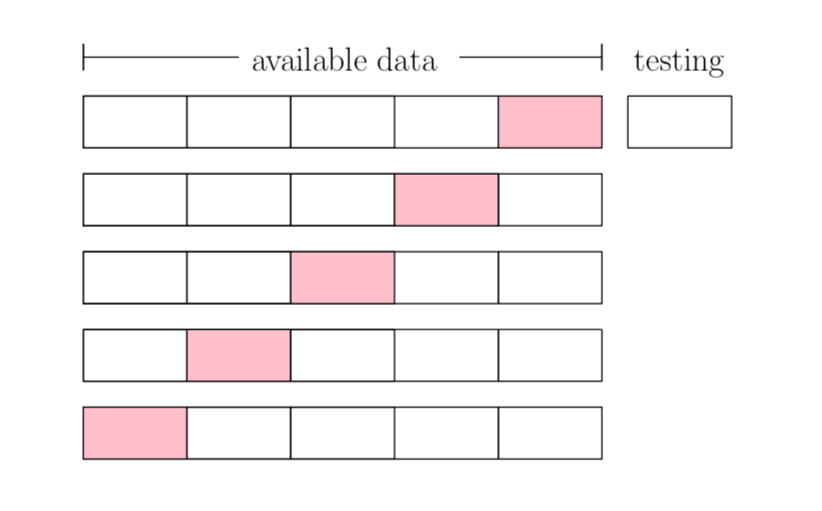
\includegraphics[width=8cm]{cross}
\end{figure}

    }
\begin{document}

\frame{\titlepage}


\begin{frame}{Scoring}

    Many possibilities are available to evaluate the quality of an estimator.
    
\end{frame}

\subsection{Regression}%
\label{sub:regression}


\begin{frame}{Regression}

    \begin{itemize}
        \item Input space $ \mathcal{X}$
        \item Output space $ \mathcal{Y}  = \mathbb{R} $.
    \end{itemize}

    Until now we used the squared error or the mean squared error (MSE):
    \begin{equation}
        MSE = \frac{1}{n} \sum^{n}_{i=1} (y_{pred, i}-y_{label, i})^2
    \end{equation}
    Without normalisation, it is also called \textbf{{residual sum of squares}} (RSS)
    \begin{equation}
        RSS = \sum^{n}_{i=1} (y_{pred, i}-y_{label, i})^2
    \end{equation}
    
\end{frame}

\begin{frame}{Coefficient of determination}

        Also called $R2$.  $R2\leq 1$. We introduce the Total sum of squares (TSS)

    \begin{equation}
        TSS = \sum^{n}_{i=1} (y_{label, i}- \bar{y})^2
    \end{equation}

    where $ \bar{y}$ is the mean of the observed data
    \begin{equation}
        \bar{y} = \frac{1}{n} \sum^{n}_{i=1} y_{label, i}
    \end{equation}
    
    Then

    \begin{equation}
        R2 = 1- \frac{RSS}{TSS} 
    \end{equation}
\end{frame}

\begin{frame}{Coefficient of determination}

    \begin{equation}
        TSS = \sum^{n}_{i=1} (y_{label, i}- \bar{y})^2
    \end{equation}

    \begin{equation}
        RSS = \sum^{n}_{i=1} (y_{pred, i}-y_{label, i})^2
    \end{equation}

    Finally we define the Explained sum of squares ESS: 

    \begin{equation}
        ESS = \sum^{n}_{i=1} (y_{pred, i}- \bar{y})^2
    \end{equation}

    Then if the predicitons are linear, then

    \begin{equation}
        TSS = ESS + RSS
    \end{equation}
    
\end{frame}

\begin{frame}{Scikit metrics}

    \url{https://scikit-learn.org/stable/modules/model_evaluation.html} 
    
\end{frame}


\subsection{Binary classification}%
\label{sub:classification}

\begin{frame}{Binary classification}

    We now review some metrics for binary classification problems.
\end{frame}


\begin{frame}{Accuracy}
   Most simple scoring: accuracy. 

   \begin{equation}
       \frac{\text{number of correct predictions}}{\text{number of samples}} 
   \end{equation}


\end{frame}

\begin{frame}{Precision and recall}

    Precision : "Quand tu dis que c'est positif, c'est positif".
    \begin{equation}
        \frac{\text{TP}}{\text{TP + FP}}       
    \end{equation}

    Recall / sensitivity (rappel) : "Quand c'est positif, tu dis que c'est positif".
    \begin{equation}
        \frac{\text{TP}}{\text{TP + FN}}
    \end{equation}

    See also: specificity and 1-specificity.
    
\end{frame}

\begin{frame}{F score}

    Also called $F1$. It quantifies the tradeoff between precision and recall.

\begin{equation}
    F1 = 2 \times \frac{\text{sensitivity}\times \text{precision}}{\text{sensitivity}+ \text{precision}} 
\end{equation}

\exercice{\textbf{}} What are the extremal values of $F$ ?

    \url{https://en.wikipedia.org/wiki/F-score} 
    
\end{frame}

\begin{frame}{Translation to french}

    In french, accuracy is sometimes translated as "précision", and precision as
    "exactitute".
    
\end{frame}


\subsection{Multi-class classification}%
\label{sub:multi_class_classification}

\begin{frame}{Binary classification}

    Standard classifiers such as logistic regression and support vector
    machines are \textbf{{binary}}. 

    However, sometimes $|\mathcal{Y} |>2$.
    
\end{frame}

\begin{frame}{Number of classifiers for multi-class classification}

    We assume $ | \mathcal{Y} | = p$.

    \exercice{\textbf{}}How many classifiers  need to be built:
    \begin{itemize}
        \item with the one-vs-rest scheme ?
        \item with the one-vs-one scheme ?
    \end{itemize}

\url{https://machinelearningmastery.com/one-vs-rest-and-one-vs-one-for-multi-class-classification/} 
\end{frame}

\begin{frame}{Number of classifiers}

    \begin{itemize}
        \item one-vs-rest is the standard approach.
        \item one-vs-one need to build a number of classifiers that is
            quadratic in $p$, ($\mathcal{O} (p^2)$).
        \item However one-vs-one might still be useful since less samples are
            used by each binary classifiers, since we only need the samples
            from the two selected classes. If the complexity of the classifier
            scales badly with the umber of samples $n$ (like for kernel
            methods), one-vs-one might be faster.
    \end{itemize}
    

\end{frame}

\begin{frame}{Scikit}

    Scikit has a builtin implementation of both schemes.

    \url{https://scikit-learn.org/stable/modules/generated/sklearn.multiclass.OneVsRestClassifier.html} 
    
\end{frame}

\begin{frame}{Softmax}

    It is also possible to directly learn $p$ real outputs and convert the vector of outputs to a probability by normalizing (it is what is done with softmax regression in neural networks).

    \url{https://fr.wikipedia.org/wiki/Fonction_softmax} 
\end{frame}

\begin{frame}{Confusion matrix}

    \url{https://en.wikipedia.org/wiki/Confusion_matrix} 

    \url{https://scikit-learn.org/stable/modules/generated/sklearn.metrics.confusion_matrix.html} 
    
\end{frame}

\begin{frame}{Classification report}

    It is also possible to define precision, recall (and thus F1) for each
    class. In scikit, classification report prints these quantities for each
    class

    \url{https://scikit-learn.org/stable/modules/generated/sklearn.metrics.classification_report.html} 
    
\end{frame}

\begin{frame}{Multi-class vs multi-label}

    Don't mix multi-class problems and multi-label problems.
    \begin{itemize}
        \item multi-class: several output classes are possible
        \item mutli-label: we have to make several predictions for each input
    \end{itemize}

    A problem can be both multi-class and multi-label.

    \url{https://scikit-learn.org/stable/modules/generated/sklearn.multioutput.MultiOutputClassifier.html} 
    \\

    Multioutput regression is also possible.

    \url{https://scikit-learn.org/stable/modules/generated/sklearn.multioutput.MultiOutputRegressor.html} 
    
\end{frame}

\subsection{Cross-validation}%
\label{sub:cross_validation}

\begin{frame}{Hyperparameters}

    All learning algorithms have hyperparameters. Examples:
    \begin{itemize}
        \item regularization parameter 
        \item learning rate schedule
        \item kernel widths
	\item tree depth for cart (trees)
        \item number of trees for random forest
    \end{itemize}
    
\end{frame}

\begin{frame}{Hyperparameter tuning}

    Sometimes, we have theoretical results that guarantee that a hyperparameter
    value is a good choice (e.g. the learning rates for GD, SGD, SAG).

    \textbf{{However:}} 
    \begin{itemize}
        \item often, these parameters values depend on constants that are
            problem-dependent and sometimes not available:
            \begin{itemize}
                \item variance $ \sigma^2$
                \item smoothness constant $L$
            \end{itemize}
        \item we may not have a theoretical result at all (true for some
            aspects of deep learning)
        \item some values of the hyperparameter might work \textbf{{better}}
            than the theoretical value.
    \end{itemize}
\end{frame}

\begin{frame}{Hyperparameter tuning}

    \textbf{{Conclusion: }} it is most often necessary to experiment and test in order to find
    relevant hyperparameters.
    
\end{frame}

\begin{frame}
    Common practice is to  test several hyperparameters, which means training several models. 
    The dataset can be split into 3 parts:

    \begin{itemize}
        \item \textbf{train set}: used to optimize each model
        \item \textbf{validation set}: used to compute a validation error of each model
            (error on this dataset). The model with lowest validation error can
            be chosen.
        \item \textbf{test set}: used to test the final model. We can not use it to
            choose the hyperparameters, otherwise the hyperparameters could "overfit this set".
	\item sometimes people use the opposite convention between "test" and "validation".
    \end{itemize}

    \textbf{{Problem}} : there might be a high variability in the validation
    procedure. The found hyperparameters might depend a lot on the initial
    choice of the validation set.
    
\end{frame}

\begin{frame}{Cross-validation}

    Cross-validation is another method that allows the use of more
    training data. The train set is split in $k$ folds (often $5$ of $10$), and
    $k$ validation errors are computed (one for each fold). The model with the
    lowest average validation error is chosen, \textbf{{and then}} trained on
    the whole train set.
    
    \begin{figure}[htpb]
        \centering
        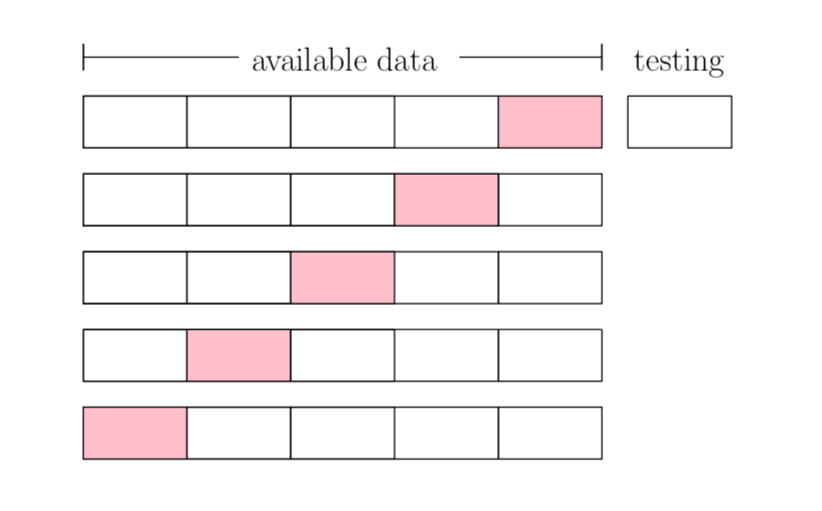
\includegraphics[width=0.5\linewidth]{cross}
        \label{fig:cross}
    \end{figure}

    Example in \textbf{3 \textunderscore validation \textunderscore cross\textunderscore validation/}

\end{frame}

\begin{frame}{Cross-validation}

    Due the the higher number of computations, cross-validation might be slower
    than standard train/validation/test split.
    
\end{frame}

\begin{frame}{Scikit}

    Grid search is a method for testing hyper parameters (exhaustive search
    among a fiven list of values).

    Grid search and cross validation are builtin in scikit.
    
    \url{https://scikit-learn.org/stable/modules/cross_validation.html} 

    \url{https://scikit-learn.org/stable/modules/generated/sklearn.model_selection.GridSearchCV.html} 
    
\end{frame}

\begin{frame}{Learning curves}

    \url{https://scikit-learn.org/stable/auto_examples/model_selection/plot_learning_curve.html} 

    Many model selection methods exist:

    \url{https://scikit-learn.org/stable/model_selection.html} 
    
\end{frame}


%% \section{Local methods}%
%% \label{sec:local_averaging}
%% \frame{\tableofcontents[currentsection]}
%% 
%% \begin{frame}{Local averaging}
%%     
%% \end{frame}
%% 
%% \subsection{Nearest neighbors}%
%% \label{sub:nearest_neighbors}
%% 
%% \begin{frame}{Nearest neighbors}
%%     
%% \end{frame}
%% 
%% 
%% 
%% \subsection{Kernel density estimation}%
%% \label{sub:kernel_density_estimation}
%% 
%% \begin{frame}{Kernel density estimation}
%%     
%% \end{frame}
%% 




\end{document} 
